\section{Performance Evaluation}
\label{sec:evaluation}
In this section, the performance of the proposed low-complexity dispatching policy $\tilde{\Policy}$ is evaluated by numerical simulations.
The experiment setup and performance benchmarks are elaborated in Section \ref{subsec:setup}.
The simulation results are illustrated in Section \ref{subsec:basic}.
The sensitivity study on parameters is also applied to provide some insights on the robustness of the proposed policy in Section \ref{subsec:advance}.

\subsection{Experiment Setup}
\label{subsec:setup}
In the simulation, there are $5$ APs, $3$ edge servers and $5$ types of jobs in the system.

The time slot duration is set as $50$ milliseconds and the broadcast interval is consist of $t_{B}=20$ time slots (i.e., duration with $1$ second).
The \brlatency~is a discrete random variable with an integer support from $10$ to $16$ time slots.
The maximum uploading latency is $3$ seconds, and the distribution of $\mathbb{U}_{k,m,j}(\Xi)$  is arbitrarily generated within the integer support $\set{0, 1, \dots, \Xi}$.
The expected computation time $c_{m,j}$ is an integer uniformly generated in the range $[30,50]$ (with the unit of time slot).

Each queue for VMs on edge server is with maximum queue length $L_{max}=20$, and the arrival rate in each time slot is uniformly generated from the range $[0.02, 0.03]$ for each job type at each AP.
The discount factor $\gamma$ and the penalty weight $\beta$ is chosen as $0.95$ and $20$, respectively.
% The arrival rate is taken as small probability with enough APs in the system, and correspondingly enough edge servers for the processing.

%-----------------------------------------------------------------------%
\begin{figure}[ht]
    \centering
    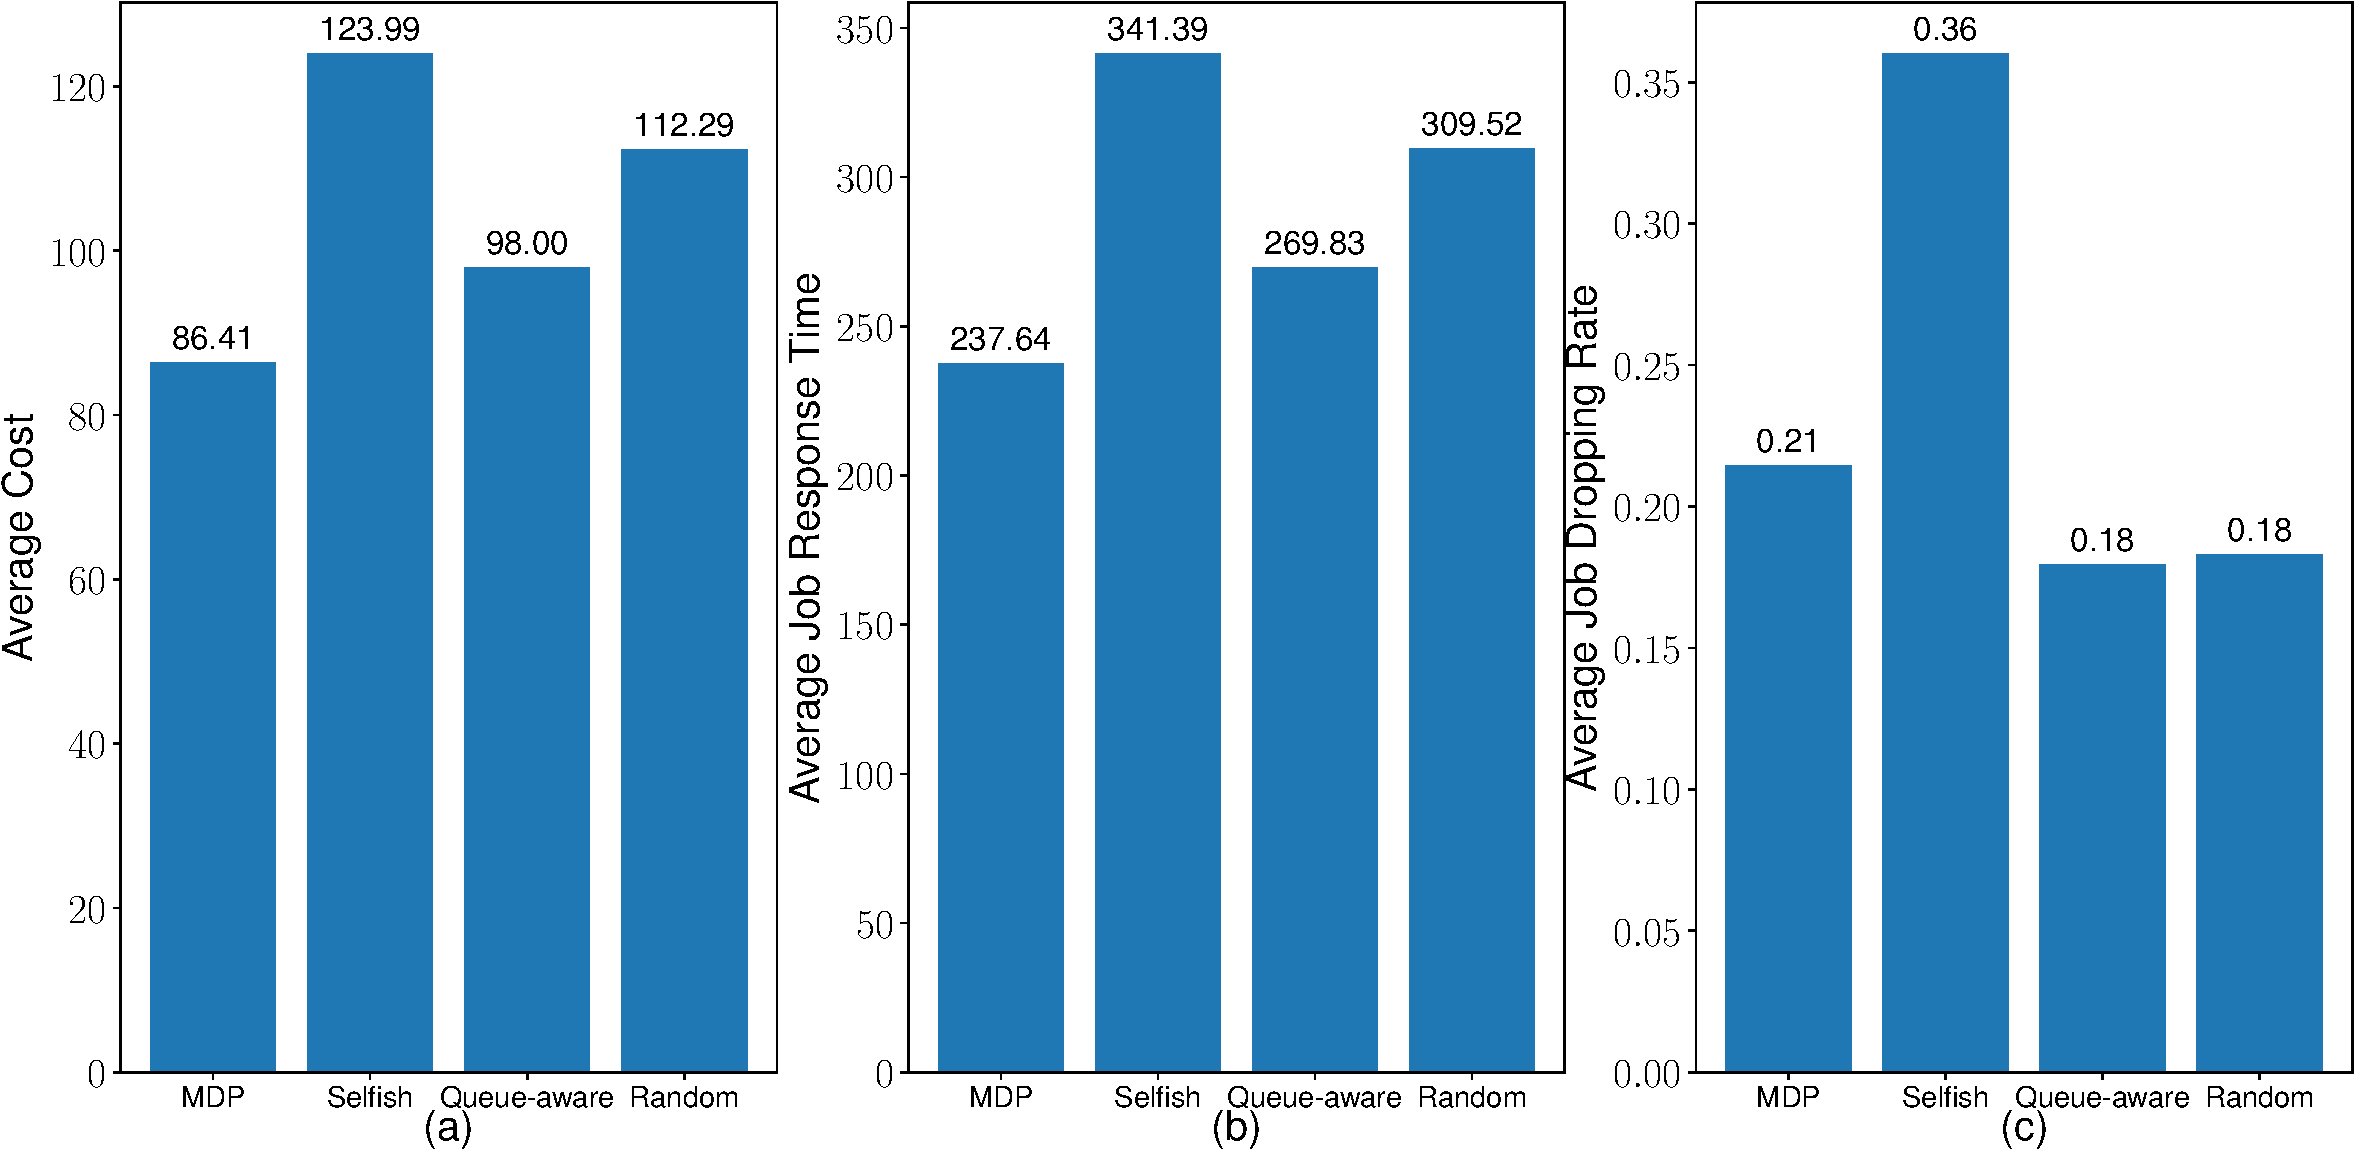
\includegraphics[width=0.90\textwidth]{41122-bar-graph-alter.pdf}
    \caption{Illustration of performance metrics comparison with various benchmarks.}
    \label{fig:bar_plot}
\end{figure}
%-----------------------------------------------------------------------%

%NOTE: Benchmark Elaboration
Various benchmarks are taken to compare with the proposed MDP policy which are listed as follows.
\begin{itemize}
    \item \textbf{Random Dispatching Policy}:
            Randomly choose a dispatching edge server in each time slot; 
    \item \textbf{Selfish Policy}:
            Always choose the edge server with the minimum sum of the expected uploading time and processing time;
    \item \textbf{Queue-aware Policy}:
            Always choose the edge server with the minimum sum of expected uploading time, processing time and queueing time based on the observation of outdated queue states.
\end{itemize}
Moreover, the Selfish Policy is taken as the initial dispatching action for the proposed algorithm (Algorithm \ref{alg_1}).
%NOTE: Basic Performance
\subsection{Performance Analysis}
\label{subsec:basic}
As illustrated in Fig.\ref{fig:bar_plot}(a), the proposed algorithm (MDP Policy) outperforms all the benchmarks in the average system cost.
Moreover, the Queue-aware Policy has better performance than the other benchmarks due to its capability of adapting dispatching action according to the outdated observation of queueing state.
More insights on the performance comparison are provided in Fig.\ref{fig:bar_plot}(b) and (c).
In the former figure, the average job response times, measuring the average number of broadcast intervals from job's arrival at one AP to the completeness of computation at one edge server, are compared.
It can be observed that the proposed policy still outperforms all the benchmarks.
In Fig.\ref{fig:bar_plot}(c), the job dropping rates, measuring the ratio of jobs dropped by edge servers due to queue overflow, are also compared.
It is shown that the proposed policy can process the approximately the same number of jobs as Queue-aware Policy and Random Policy, while with the minimum average cost and job response time.

\subsection{Sensitivity Study}
\label{subsec:advance}  

%FIXME: replace the graphs
%-----------------------------------------------------------------------------------%
\begin{center}
    \begin{figure*}[ht!]
        \begin{tabular}{ccc}
            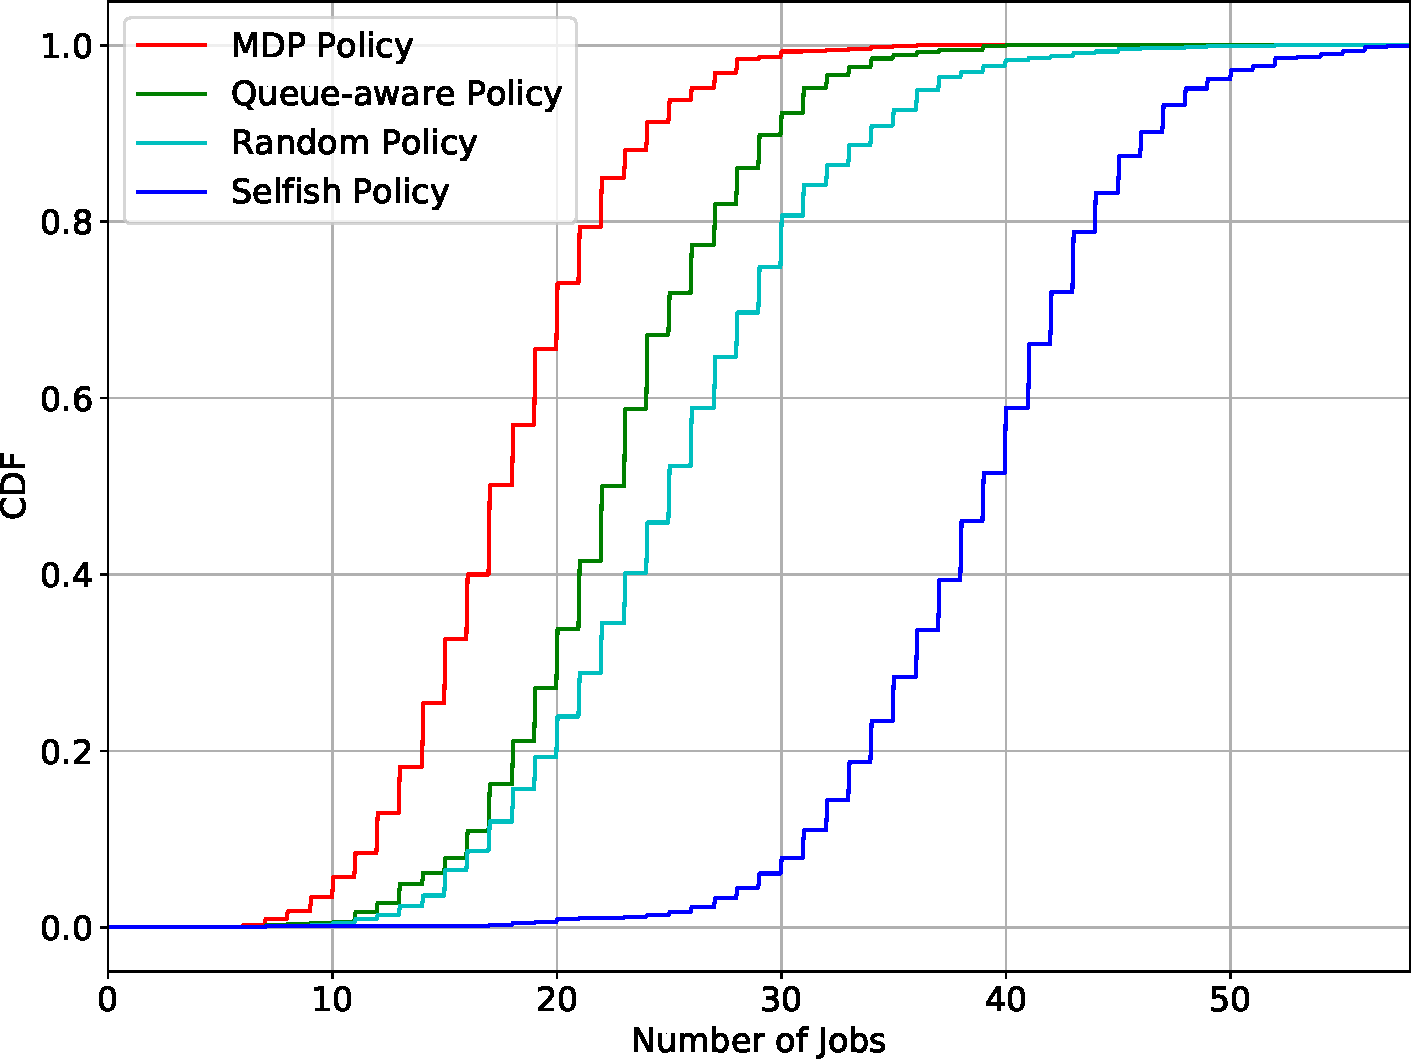
\includegraphics[width=0.30\textwidth]{LowPressure-d0.pdf}&
            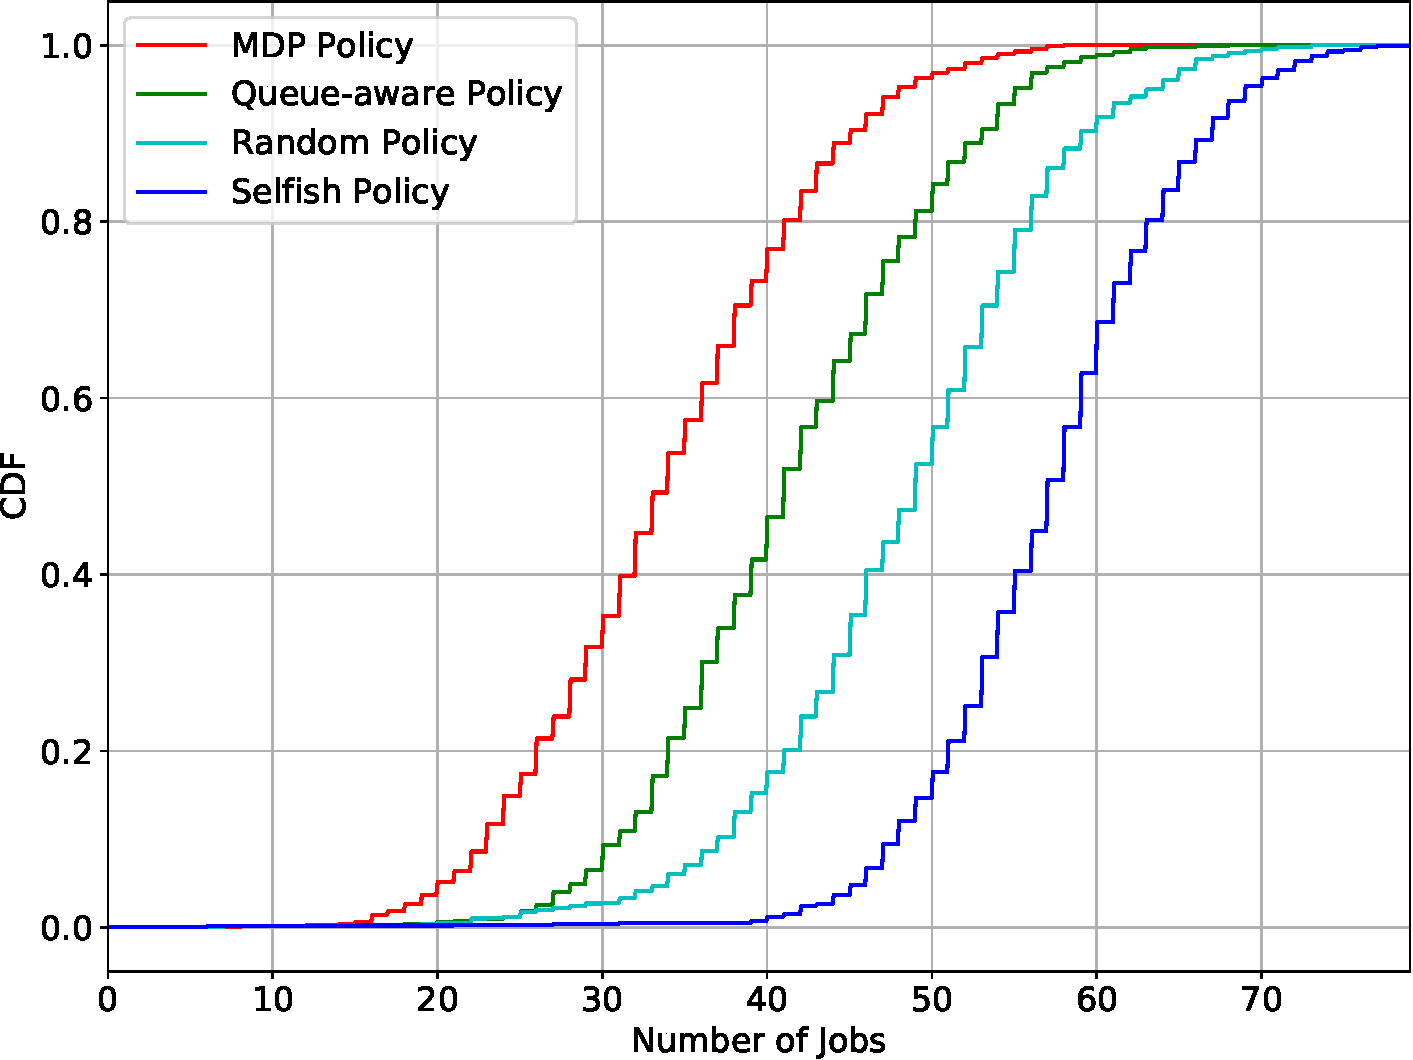
\includegraphics[width=0.30\textwidth]{LowPressure-d1.pdf}&
            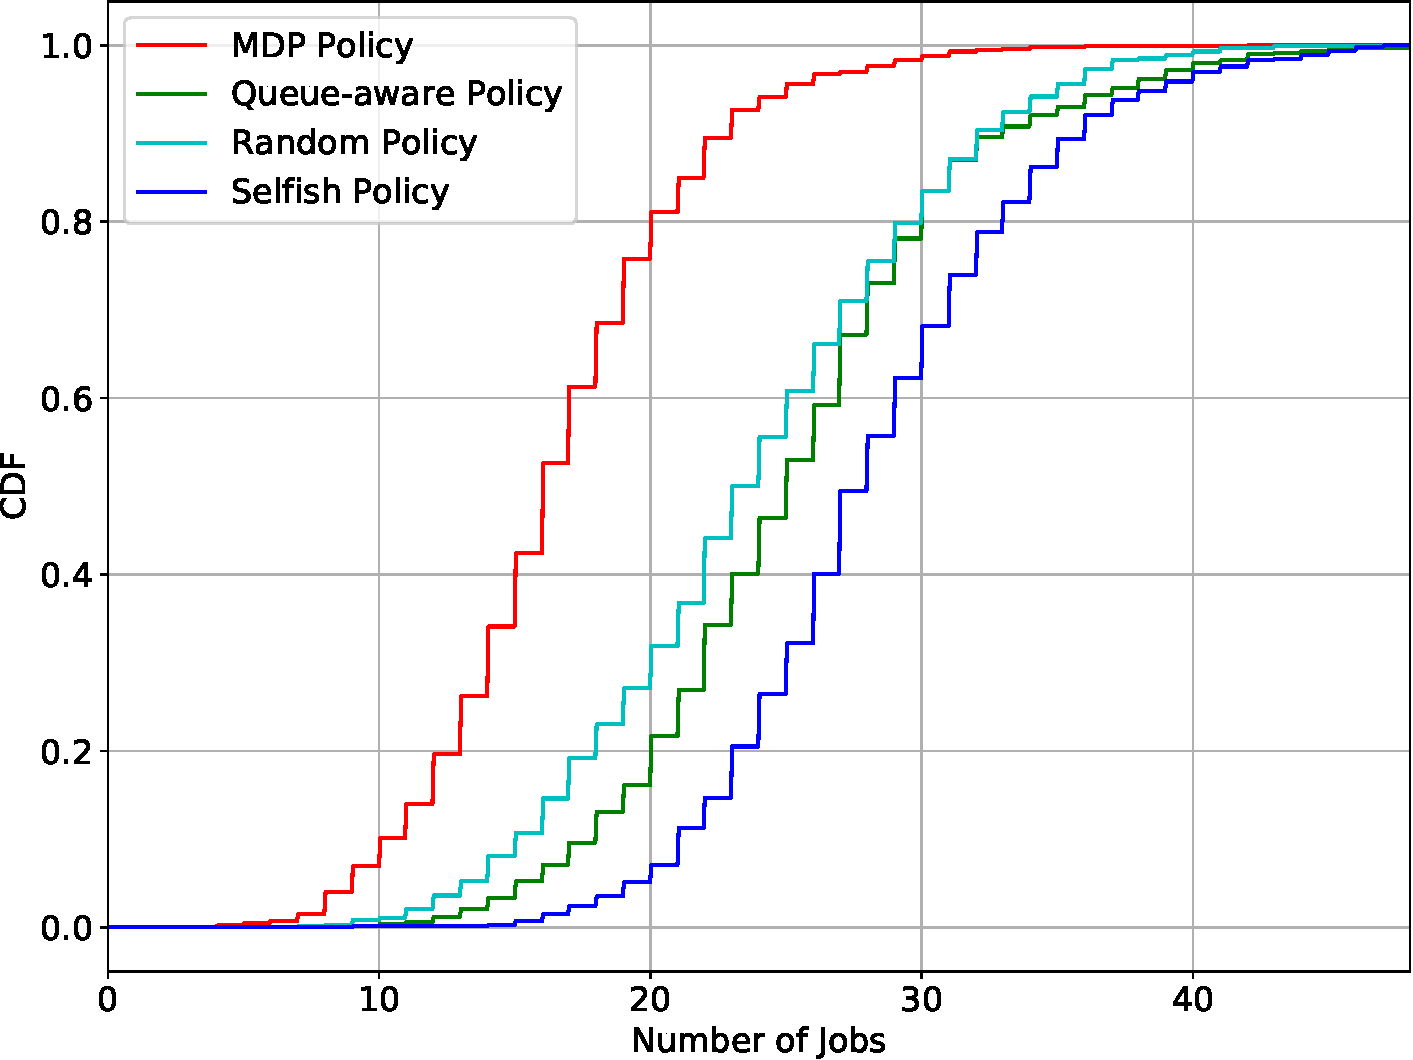
\includegraphics[width=0.30\textwidth]{LowPressure-d2.pdf}
            \\
            {\small (a) Zero \brlatency} &
            {\small (b) Signaling latency with Support $\set{10,\dots,16}$} &
            {\small (c) Maximum \brlatency}
        \end{tabular}
        \caption{Illustration of Sensitivity Study on Algorithm Robustness versus Signaling Latency.}
        \label{fig:ss_signal}
    \end{figure*}
\end{center}
%-----------------------------------------------------------------------------------%

%TODO: tabular the figures here
\begin{figure}[htbp]
    \begin{minipage}[t]{0.45\linewidth}
        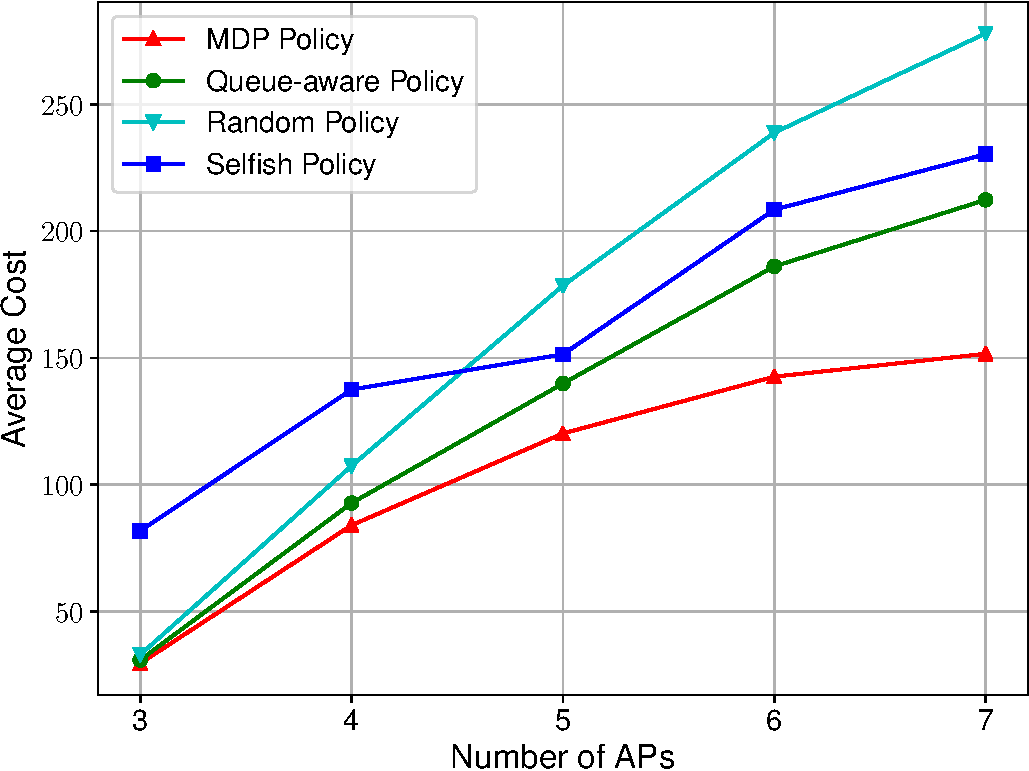
\includegraphics[width=\linewidth]{Study-NumAPs.pdf}
        \caption{Illustration of Sensitivity Study on Average System Cost versus the Number of APs.}
        \label{fig:ss_scale}
    \end{minipage}
    \hfill
    \begin{minipage}[t]{0.45\linewidth}
        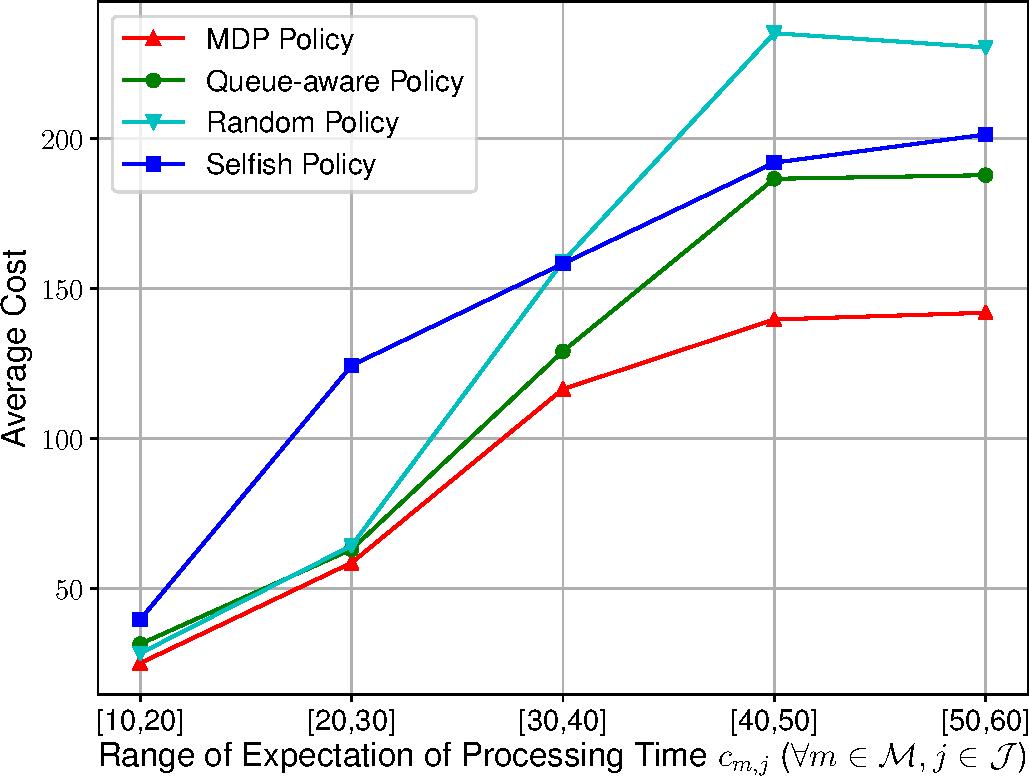
\includegraphics[width=\linewidth]{Study-ProcDist.pdf}
        \caption{Illustration of Sensitivity Study on Average System Cost versus the Processing Time Distributions.}
        \label{fig:ss_dist}
    \end{minipage}
\end{figure}

%NOTE: sensitivity study
\textbf{Signaling Latency.}
The simulation results with different distributions of \brlatency~$\mathcal{D}_{k}$ ($\forall k\in\apSet$) are illustrated in Fig.\ref{fig:ss_signal}, where the cumulative distribution function (CDF) of the job number in the system is plotted.
Specifically, the \brlatency~of all the APs is set to zero and $20$ time slots in Fig.\ref{fig:ss_signal}(a) and Fig.\ref{fig:ss_signal}(c), respectively, and the \brlatency~is a random variable with integer support from $10$ to $16$ time slots in Fig.\ref{fig:ss_signal}(b).
It can be observed from Fig.\ref{fig:ss_signal}(a) and Fig.\ref{fig:ss_signal}(c) that, with the increasing \brlatency, the performance of Queue-aware Policy becomes worse.
It outperforms Random Policy in Fig.5(a) with zero \brlatency~(achieving a smaller number of jobs in the system), and becomes worse in Fig.5(c) with large \brlatency.
This demonstrates that the Queue-aware Policy is sensitive to the \brlatency.
In all the figures, the proposed policy performs better than the benchmarks, which demonstrates the robustness of its performance versus signaling latency.

\textbf{Number of APs.} %(a.k.a arrival rate)
The average system cost versus the number of APs is illustrated in Fig.\ref{fig:ss_scale}.
With the increasing AP numbers, the average system cost increases in all the benchmarks and the proposed policy.
It can be observed that the proposed policy has better performance than the benchmarks for all numbers of APs.
Moreover, the performance gain becomes significant when the computation load is heavy ($K$ is large).
This demonstrates the dispatching efficiency of the proposed policy with heavy load.
On the other hand, the gain is negligible for light load ($K=3$), where the computation capability is sufficient and dispatcher optimization may not be necessary.

\textbf{Processing Time Distributions.}
The simulation results of various distributions of processing time are illustrated in Fig.\ref{fig:ss_dist}, where the $c_{m,j}$ of the processing time distribution $\mathbb{G}(1/c_{m,j})$ ($\forall m\in\esSet,j\in\jSpace$) is generated within different ranges.
Generally speaking, with the increasing average processing time, the average system cost increases in all the benchmarks and the proposed policy.
The simulation results are consistent with that in Fig.\ref{fig:ss_scale}.
It can be observed that the proposed policy has better performance than the benchmarks.
Moreover, the performance gain becomes significant when the computation time is long (the computation load is heavy).
On the other hand, the gain is negligible for short computation time (the computation load is light).

%----------------------------------------------------------------------------------------%
%----------------------------------------------------------------------------------------%
